% Template for ICASSP-2013 paper; to be used with:
%          spconf.sty  - ICASSP/ICIP LaTeX style file, and
%          IEEEbib.bst - IEEE bibliography style file.
% --------------------------------------------------------------------------
\documentclass{article}
\usepackage{spconf,amsmath,graphicx}

% Example definitions.
% --------------------
\def\x{{\mathbf x}}
\def\L{{\cal L}}

% Title.
% ------
\title{AUTHOR GUIDELINES FOR ICASSP 2014 PROCEEDINGS MANUSCRIPTS}

%
% Single address.
% ---------------
\name{Author(s) Name(s)\thanks{Thanks to XYZ agency for funding.}}
\address{Author Affiliation(s)}
%
% For example:
% ------------
%\address{School\\
%   Department\\
%   Address}
%
% Two addresses (uncomment and modify for two-address case).
% ----------------------------------------------------------
%\twoauthors
%  {A. Author-one, B. Author-two\sthanks{Thanks to XYZ agency for funding.}}
%   {School A-B\\
%   Department A-B\\
%   Address A-B}
%  {C. Author-three, D. Author-four\sthanks{The fourth author performed the work
%   while at ...}}
%   {School C-D\\
%   Department C-D\\
%   Address C-D}
%
\begin{document}
%\ninept
%
\maketitle
%
\begin{abstract}
Transitions between stable states are the dominant mechanism for biological function
at the molecular level.  A full molecular understanding of how these transitions are
driven remains a challenging problem due to the high dimensionality of the protein
space and the poor sampling that is achieved with modern molecular dynamics simulations.
We argue in this paper that a streaming database with machine learning algorithms
to enable feature engineering, dimensionality reduction, and state identification can
be used to define the most important degrees of freedom that drive conformational
change. Our algorithm is tested on BPTI using the data generated from the DE Shaw
research group as an initial entry point for classification of states and an initial
description of the events leading to transitions between states.
\end{abstract}
%
\begin{keywords}
One, two, three, four, five
\end{keywords}
%
\section{Introduction}
\label{sec:intro}

Many years of research has shown that proteins live in a multi-time scale universe
with long dwell times in stable states separated by rapid transitions between states.
Structural work has confirmed that many proteins have a stable state that can be
solved by x-ray or nmr methods.  Further experimental work on several canonical
systems has been able to prove the existence of alternative stable structures.  A
full, experimental, characterization of the transitions between folded states is,
in general, an intractable problem that has resisted a general solution.

Molecular dynamics can be a tremendous aid for such settings, by providing
a detailed molecular view of the stable states and their nearby stable conformational
wells.  Despite the promise of molecular dynamics as a general solution for understanding
the functional significance of conformational change, the computational limits of
sampling have prevented, even in the best of cases, a fully detailed description of
all states and samples on the transitions between states have been even more
difficult to obtain in a converged manner.  

This paper is an attempt to understand more about state to state conformational
change by first using machine learning methods to better understand the features
that describe the states and then to couple that knowledge to enable an iterative
sampling approach to be defined that enables a more rapid and more confident
convergence on the transitions between states.



\section{Formatting your paper}
\label{sec:format}


\section{PAGE TITLE SECTION}
\label{sec:pagestyle}


\section{TYPE-STYLE AND FONTS}
\label{sec:typestyle}


\section{MAJOR HEADINGS}
\label{sec:majhead}


\subsection{Subheadings}
\label{ssec:subhead}


\subsubsection{Sub-subheadings}
\label{sssec:subsubhead}

Sub-subheadings, as in this paragraph, are discouraged. However, if you
must use them, they should appear in lower case (initial word
capitalized) and start at the left margin on a separate line, with paragraph
text beginning on the following line.  They should be in italics.

\section{PRINTING YOUR PAPER}
\label{sec:print}

Print your properly formatted text on high-quality, 8.5 x 11-inch white printer
paper. A4 paper is also acceptable, but please leave the extra 0.5 inch (12 mm)
empty at the BOTTOM of the page and follow the top and left margins as
specified.  If the last page of your paper is only partially filled, arrange
the columns so that they are evenly balanced if possible, rather than having
one long column.

In LaTeX, to start a new column (but not a new page) and help balance the
last-page column lengths, you can use the command ``$\backslash$pagebreak'' as
demonstrated on this page (see the LaTeX source below).

\section{PAGE NUMBERING}
\label{sec:page}

Please do {\bf not} paginate your paper.  Page numbers, session numbers, and
conference identification will be inserted when the paper is included in the
proceedings.

\section{ILLUSTRATIONS, GRAPHS, AND PHOTOGRAPHS}
\label{sec:illust}

Illustrations must appear within the designated margins.  They may span the two
columns.  If possible, position illustrations at the top of columns, rather
than in the middle or at the bottom.  Caption and number every illustration.
All halftone illustrations must be clear black and white prints.  Colors may be
used, but they should be selected so as to be readable when printed on a
black-only printer.

Since there are many ways, often incompatible, of including images (e.g., with
experimental results) in a LaTeX document, below is an example of how to do
this \cite{Lamp86}.

\section{FOOTNOTES}
\label{sec:foot}

Use footnotes sparingly (or not at all!) and place them at the bottom of the
column on the page on which they are referenced. Use Times 9-point type,
single-spaced. To help your readers, avoid using footnotes altogether and
include necessary peripheral observations in the text (within parentheses, if
you prefer, as in this sentence).

% Below is an example of how to insert images. Delete the ``\vspace'' line,
% uncomment the preceding line ``\centerline...'' and replace ``imageX.ps''
% with a suitable PostScript file name.
% -------------------------------------------------------------------------
\begin{figure}[htb]

\begin{minipage}[b]{1.0\linewidth}
  \centering
  \centerline{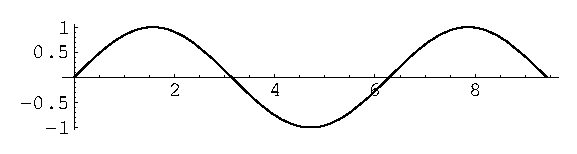
\includegraphics[width=8.5cm]{image1}}
%  \vspace{2.0cm}
  \centerline{(a) Result 1}\medskip
\end{minipage}
%
\begin{minipage}[b]{.48\linewidth}
  \centering
  \centerline{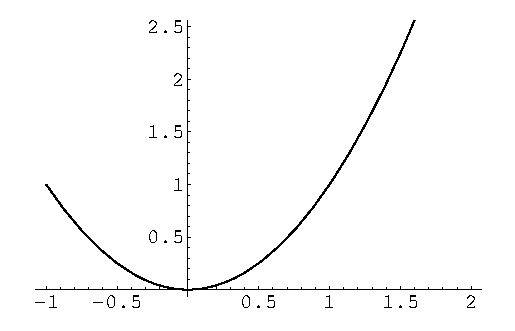
\includegraphics[width=4.0cm]{image3}}
%  \vspace{1.5cm}
  \centerline{(b) Results 3}\medskip
\end{minipage}
\hfill
\begin{minipage}[b]{0.48\linewidth}
  \centering
  \centerline{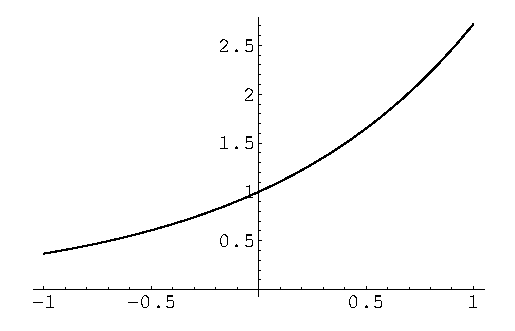
\includegraphics[width=4.0cm]{image4}}
%  \vspace{1.5cm}
  \centerline{(c) Result 4}\medskip
\end{minipage}
%
\caption{Example of placing a figure with experimental results.}
\label{fig:res}
%
\end{figure}


% To start a new column (but not a new page) and help balance the last-page
% column length use \vfill\pagebreak.
% -------------------------------------------------------------------------
%\vfill
%\pagebreak

\section{COPYRIGHT FORMS}
\label{sec:copyright}

You must submit your fully completed, signed IEEE electronic copyright release
form when you submit your paper. We {\bf must} have this form before your paper
can be published in the proceedings.

\section{RELATION TO PRIOR WORK (NEW)}
\label{sec:prior}

The text of the paper should contain discussions on how the paper's
contributions are related to prior work in the field. It is important
to put new work in  context, to give credit to foundational work, and
to provide details associated with the previous work that have appeared
in the literature. This discussion may be a separate, numbered section
or it may appear elsewhere in the body of the manuscript, but it must
be present.

You should differentiate what is new and how your work expands on
or takes a different path from the prior studies. An example might
read something to the effect: "The work presented here has focused
on the formulation of the ABC algorithm, which takes advantage of
non-uniform time-frequency domain analysis of data. The work by
Smith and Cohen \cite{Lamp86} considers only fixed time-domain analysis and
the work by Jones et al \cite{C2} takes a different approach based on
fixed frequency partitioning. While the present study is related
to recent approaches in time-frequency analysis [3-5], it capitalizes
on a new feature space, which was not considered in these earlier
studies."

\vfill\pagebreak

\section{REFERENCES}
\label{sec:refs}

List and number all bibliographical references at the end of the
paper. The references can be numbered in alphabetic order or in
order of appearance in the document. When referring to them in the
text, type the corresponding reference number in square brackets
as shown at the end of this sentence \cite{C2}. \textbf{An
additional final page (the fifth page, in most cases) is allowed,
but must contain only references to the prior literature.}

% References should be produced using the bibtex program from suitable
% BiBTeX files (here: strings, refs, manuals). The IEEEbib.bst bibliography
% style file from IEEE produces unsorted bibliography list.
% -------------------------------------------------------------------------
\bibliographystyle{IEEEbib}
\bibliography{strings,refs}

\end{document}
